\documentclass[fleqn,10pt]{wlscirep}
\usepackage[utf8]{inputenc}
\usepackage{pst-all}
\usepackage{hyperref}
\usepackage[hidelinks]{hyperref}
\usepackage{float}
\usepackage{xfrac}
\usepackage{longtable}
\usepackage{subcaption}
\usepackage{multicol}
\usepackage{amsmath,amsfonts,amssymb,amsthm}
\usepackage{url}
\usepackage{bbm}
\usepackage{subcaption}
\usepackage{listings}
\usepackage{mwe}
\usepackage{breqn}
\usepackage{amsthm}
\newtheorem{theorem}{Theorem}

\makeatletter
\renewcommand*\env@matrix[1][c]{\hskip -\arraycolsep
  \let\@ifnextchar\new@ifnextchar
  \array{*\c@MaxMatrixCols #1}}
\makeatother

\theoremstyle{definition}
\newtheorem{definition}{Definition}

\lstset{
  basicstyle=\ttfamily,
  mathescape
}
\setlength{\belowcaptionskip}{-0.2cm}
\arraycolsep=1.4pt
\def\arraystretch{2} 
\usepackage{mathtools}
\DeclarePairedDelimiter{\ceil}{\lceil}{\rceil}
\title{Analysis of fractional-order system for financial dynamics}
\let\iif\leftrightarrow
\author[1]{Mateo Restrepo Sierra}
\author[2]{Juan S. C\'ardenas Rodr\'iguez}
\author[3]{David Plazas Escudero}
\affil[1]{Universidad EAFIT, mrestrepos@eafit.edu.co, Student, Medell\'in, Colombia}
\affil[2]{Universidad EAFIT, jscardenar@eafit.edu.co, Student, Medell\'in, Colombia}
\affil[3]{Universidad EAFIT, dplazas@eafit.edu.co, Student, Medell\'in, Colombia}
\keywords{Macroeconomic financial system, fractional-order system, chaos, stability, feedback control, Adams-Bashforth-Moulton algorithm.}

 \begin{abstract}
	This work studies the Huang-Li financial nonlinear dynamic system, based on Chen's generalization: the given system can be also studied for non-integer order differential equations. This approach is based on two main facts that involves financial systems: chaos and memory. In one hand, it can be shown that the dynamic system in study is indeed a chaotic system; on the other hand, as financial systems are highly correlated with previous events, memory is essential, hence the use of fractional derivatives. A stability analysis and control were performed. This work is intended to give a more detailed version of the procedure mentioned in Chen's paper, since all simulation parameters for the system are specified and we include a short comparison between the numerical procedures. It was found that the system is highly controllable in both equilibrium points and periodic orbits; the stability of some points is strongly dependent on the system's order. On the other hand, a sensitivity analysis was done based on methods described on the literature and it was found that the system is sensitive to different parameters depending on the order.
 \end{abstract}
\begin{document}

\flushbottom
\maketitle

\thispagestyle{empty}

\section{Introduction}
In the 1920s, Charles Ponzi duped investors when he convinced them that he will return a 50\% revenue every 90 days; he was actually paying the old investors with the money given by the new ones. This is known as the Ponzi Scheme nowadays; since the virtual currencies lack of regulation and have enhanced privacy for trading, they can be and are being used by fraudsters to perpetrate their frauds in similar fashion \cite{ponzi}.

\noindent In 2017, the cryptocurrency company BitConnect launched its new coin BitConnect Coin (BCC, not to be confused with BitCoin Cash), which assured every user that whatever investment they made in their currency and made part of their loan and exchange platform (which allowed them to loan the company USD and Bitcoin to the company in favor of some interests) they will return up to 40\% of their initial investment every month. After using broad marketing strategies to avoid their investors to know about their fraudulent intentions and recollecting thousands of investments, they closed the loan and exchange platform; so, all the people who invested in the BCC lost all their money because of the 96\% drop in the price of the coin. Even the company promised to return some money for the people who got affected by given them the average of the price of the coin in the last 15 days but, given that BCC was at such a low price there were several financial lossess by the investors. In this day and age, there are new companies like XRPConnect, EthConnect, Bunny Token and NEOConnect that are replicating the schemes that BCC made without any type of regulation which, as what happened with BitConnect, can lead to disastrous results \cite{nextWeb}.

\noindent In this manner, cryptocurrencies can over-inflate their price by artificially manipulating the price by marketing it with unrealistic expectations so people start buying the coin and in some delay, selling it to other people to obtain profit through the Exchanges or the Peer to Peer system, who would put more coins in the market through mining. As they exploit the price and people invest more in the coin, they then can abuse this by incrementing by a big margin their Exchange rate or, on the other side, the company changes the coins it possesses for USD or another currency and, proceed to devaluate their coin so they do not have to pay people back. \cite{bcc11}.

\noindent On the other hand, price leveraging is not as hard in cryptocurrencies as other stocks that are available in the market. An article written in the Journal of Monetary Economics about the price manipulation in the bitcoin system, that the sudden spike in the price of bitcoin in 2013 happened due to suspicious activity in an exchanges called ``Mt.Gox Bitcoin Currency Exchange'', which 600000 BTC valued at 188 million USD were acquiered using bots, artificially inflating the price without any real substance; the article explains how this could have a massive effect in the growth rate of BTC in a positive manner, reaching a 4\% growth rate each day after \cite{PMitBE}.

\subsection{Problem of cryptocurrencies}
Taking account of all the above, the cryptocurrency system allows for people to abuse it in fraudulent ways to augment the growth rate of the price of that coin without any type of repercusion, due to the lack of goverment regulation. On the other hand, as an articles of forbes says, most of investors in this currencies like this investment because of the same lack of government involvement \cite{forbes}. In this manner, nowadays companies like Bunny Token, ETH Connect, XRPConnect and mire are expecting 1\% growth in their price daily without any type of proof or security for the investors without too much control because, of the lack of control they have, leading to a easier atmosphere to scam people.

\indent To conclude, it's important to notice that even if the problem and the variables have a very short span, there can be found a lot of documentation about them because they were one of the trending topics last year. Most people see Bitcoin and other cryptocurrencies as a safe economic investment and a way to make easy profit. Although we are not saying that is something that we should thrive to eliminate completely, it is important to examine how this system works and start to make policies that makes investing in this opportunity a safer place for the consumer and, stop catastrophes like BitConnect to don't ever happen again.



\section{Methodology}
  \subsection{System Description}
    The system chosen for this work is taken from Chen's generalization in \cite{main}, but was originally proposed by Huang \& Li in \cite{huang1993theory}. In this paper, both approaches will be studied. The dynamic system was originally proposed as a first order differential equations system, but Chen's claims this can be generalized for fractional-order differential equation system. Thus, the systems are
    \begin{equation}
        \begin{array}{ll}
            \dot{X}&=Z+(Y-a)X\\
            \dot{Y}&=1-bY-X^2\\
            \dot{Z}&=-X-cZ\\
            &\textit{Original}
        \end{array}\qquad\Rightarrow\qquad
        \begin{array}{ll}
            \dfrac{d^{q_1}X}{dt^{q_1}}&=Z+(Y-a)X\\
            \dfrac{d^{q_2}Y}{dt^{q_2}}&=1-bY-X^2\\
            \dfrac{d^{q_3}Z}{dt^{q_3}}&=-X-cZ\\
            &\textit{Generalized}
        \end{array} \qquad q_1,q_2,q_3\in(0,1]
        \label{eq:main}
    \end{equation}
    This financial system describes the behavior of three state variables (i.e. $X$, $Y$, $Z$), which are respectively the interest rate, the investment demand and the price index; $a$, $b$ and $c$ are non-negative parameters that have real interpretation, these are (respectively): savings, cost per investment, elasticity of demand. We will give a short definition for each concept:
    \begin{itemize}
    \item Interest rate ($X$): is the cost of borrowed money, expressed as a percentage of the loan amount \cite{interestRate}.
    \item Investment demand($Y$): ``investment demand refers to the demand by businesses for physical capital goods and services used to maintain or expand its operations'' \cite{investmentDemand}.
    \item Price index ($Z$): measure of relative price changes \cite{priceIndex}.
    \item Savings ($a$): ``is what a person has left over when the cost of his or her consumer expenditure is subtracted from the amount of disposable income earned in a given period of time'' \cite{savings}.
    \item Cost per investment ($b$): also known as pre-operative cost, it is the necessary cost that we incurred in order to start an specific project.
    \item Elasticity of demand ($c$): ``measure of variable reaction to a change in another variable'' If  $c < 1$ is inelastic, in the other case is elastic \cite{elasticity}.
    \end{itemize}

	Previous studies claim that these equations (\ref{eq:main}) were obtained through analysis and a considerable number of experiments:
    \begin{itemize}
    \item $X$ comes from two important facts: first, the investment and savings are inversely proportional, and last the adjustment goods prices.
    \item $Y$ is in proportion with the rate of investment, and in proportion to inversion with the cost of investment and the the interest rate.
    \item The price index $Z$ depends on the inverse relationship between supply and demand of the commercial market; furthermore is related with the inflation rate. This is supposing that the amount of supplies and demands are constant\cite{jun2001study}. 
    \end{itemize}

	\subsection{Mathematical Model}
    
      Recall the dynamic system
      \begin{equation}
          \begin{array}{ll}
              \dfrac{d^{q_1}X}{dt^{q_1}}&=Z+(Y-a)X\\
              \dfrac{d^{q_2}Y}{dt^{q_2}}&=1-bY-X^2\\
              \dfrac{d^{q_3}Z}{dt^{q_3}}&=-X-cZ\\
          \end{array}
      \end{equation}
      For the original approach (i.e. integer order), will be treated as a specific case of the generalized model when  $q_1=q_2=q_3=1$. For the generalized model, since there are many definitions for fractional-order derivatives, the same definition as in Chen's paper will be used. Therefore, let us define the Caputo-type fractional derivative as 
      \begin{equation}
      	\dfrac{d^\alpha y}{dx^\alpha} = D_*^\alpha y(x) =  J^{m-\alpha}y^{(m)}(x), \quad \alpha > 0
      \end{equation}
      Where $m=\ceil{\alpha}$ is the ceil function of $\alpha$, $y^{(m)}$ is the $m$th ordinary derivative of $y$ and $J^{m-\alpha}$ is the Riemann-Liouville integral operator of order $m-\alpha$. This last operator is defined as
      \begin{equation}
      	J^\beta z(x) = \frac{1}{\Gamma (\beta)}\int_0^\infty{(x-t)^{\beta-1}z(t)dt}, \quad \beta > 0
      \end{equation}
      and $\Gamma(\beta)$ is the gamma function. For solving fractional differential equations, the Adams-Bashforth-Moulton predictor-corrector is used for numerical solutions; this method, introduced in \cite{diethelm2002predictor}, is presented in section \ref{sec:adam}.
      \subsection{Block Diagram}
      The following block diagram is only for the integer-order system with MathWork's Simulink, since the fractional order system was solved using Adams-Bashforth-Moulton predictor-corrector, in a standard Matlab script.
      
      \begin{figure}[H]
      	\centering
        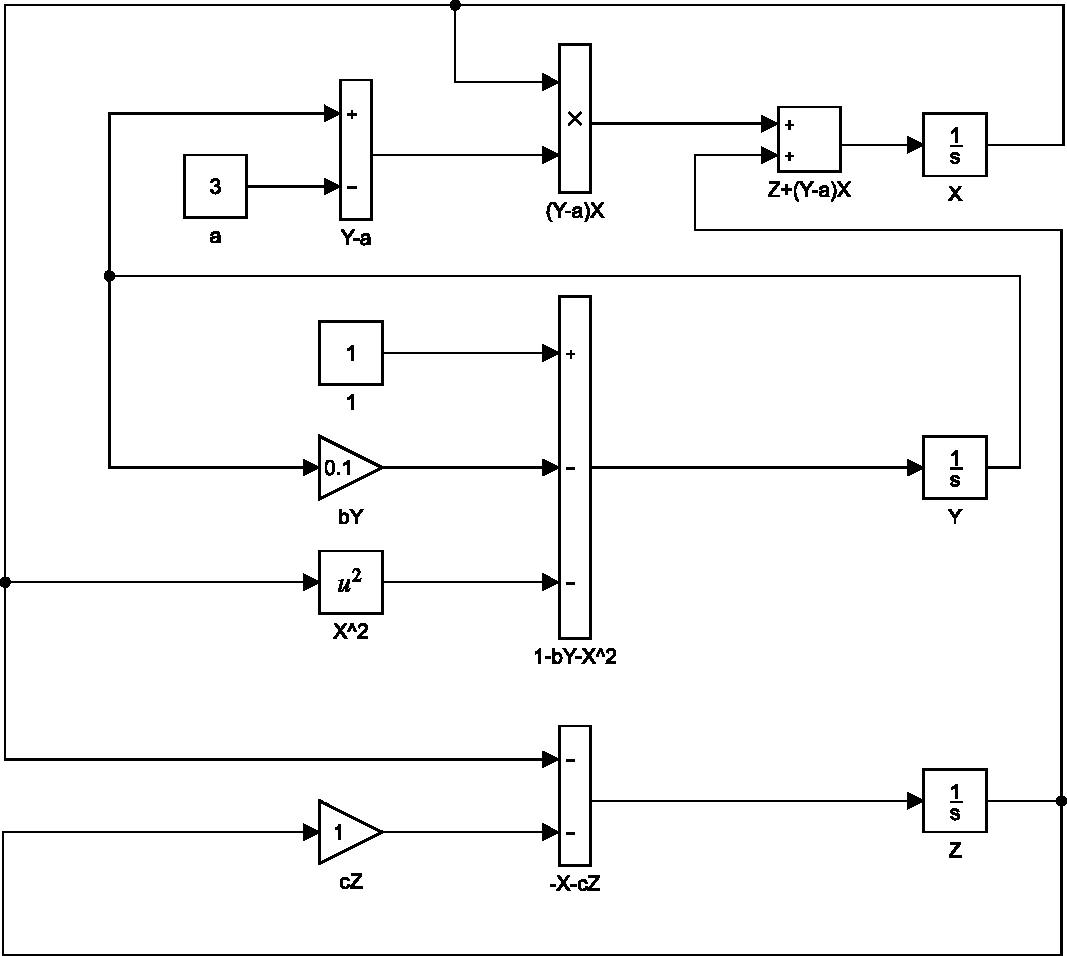
\includegraphics[scale=0.5]{files/DiagramaBloques.pdf}
        \caption{Block diagram for integer-order system.}
        \label{fig:block}
      \end{figure}
      
      \subsection{Simulation Method}
		\subsubsection{Adams-Bashforth-Moulton Algorithm}
        \label{sec:adam}
		Here the pseudo-code of the algorithm will be presented as in \cite{diethelm2002predictor}, this algorithm is applied to approximate the solution of a fractional differential equation 
        \begin{equation}
        	D_*^\alpha y(x) = f(x,y(x))
        \end{equation}
        
         where where $\alpha>0$ is the order of the differential equation, on a interval $[0,T]$.\\
        
        INPUT VARIABLES
        
        \begin{equation*}
        	\begin{array}{ll}
        		f &= \text{real-valued function defined for right side of the differential equation $D_*^\alpha y(x) = f(x,y(x))$}\\
                \alpha &= \text{the order of the fractional differential equation, real and positive number}\\
                y_0 &= \text{array of $\ceil{\alpha}$ initial conditions, i.e. $y(0),y'(0),...,y^{(\ceil{\alpha}-1)}(0)$}\\
                T &= \text{positive real-valued upper limit of the approximated solution interval}\\
                N &= \text{the number of steps that the method will take in the interval}\\ 
        	\end{array}
        \end{equation*}
        
        OUTPUT        
        \begin{equation*}
        	y = \text{an array of $N+1$ real numbers that contains the approximation for each value of $T/N$ in the interval}
        \end{equation*}
        
        %\pagebreak
        
        PROCEDURE
        \begin{lstlisting}
      h = T/N
      m = $\ceil{\alpha}$
      for $k=1$ to N do
      	$b[k]=k^\alpha-(k-1)^\alpha$
        $a[k]=(k+1)^{\alpha+1}-2k^{\alpha+1}+(k-1)^{\alpha+1}$
      end
      $y[0]=y_0[0]$
      for $j=1$ to N do
      	$P=\displaystyle\sum_{k=0}^{m-1}\limits\frac{(jh)^k}{k!}y_0[0]+\frac{h^\alpha}{\Gamma(\alpha+1)}\left[\displaystyle\sum_{k=0}^{j-1}\limits b[j-k]f(kh,y[k])\right]$
        $y[j]=\displaystyle\sum_{k=0}^{m-1}\limits\frac{(jh)^k}{k!}y_0[0]+\frac{h^\alpha}{\Gamma(\alpha+2)}\left[f(jh,P)+\left((j-1)^{\alpha+1}-f(0,y(0))(j-1-\alpha)j^\alpha\right)+\displaystyle\sum_{k=0}^{j-1}\limits a[j-k]f(kh,y[k])\right]$
      end
        \end{lstlisting}
        \subsubsection{Runge-Kutta Method}
        	Given the system to solve:
            \begin{equation}
            	y' = f(x,y)
            \end{equation}
            With the initial condition $y(0)=x_0$ and a specific time period to simulate the system $h$ the fourth order Runge-Kutta method dictates that the solution:
            \begin{equation}
            	y_{i+1} = y_i + \frac{h}{6}(k_1 + 2k_2 + 2k_3 + k_4)
            \end{equation}
            With:
            \begin{equation}
			\begin{array}{ll}
            	k_1 = f(x_i, y_i) \\
                k_2 = f(x_i + \frac{h}{2}, y_i + \frac{hk_1}{2}) \\
                k_3 = f(x_i + \frac{h}{2}, y_i + \frac{hk_2}{2}) \\
                k_4 = f(x_i + \frac{h}{2}, y_i + hk_3)
    		\end{array}
\end{equation}
		Furthermore, this method has different versions due to the application of different orders of this algorithm \cite{kutta}; therefore, it would be expected that this method is more precise than the Adam-Bashforth-Moulton because is three orders less compared to Runge-Kutta when both used to solve integer derivatives. On the other hand, there is no way to use the first method to solve fractional derivatives in higher orders (at least with reasonable complexities) therefore the Adam's algorithm has more computability than the Kutta's. 
            This method was used for the specific case for integer-order model i.e. $q_1=q_2=q_3=1$.

\section{Results \& Discussion}
For all of the following simulations, we set the value of the parameters to $a=3$, $b=0.1$ and $c=1$ with the initial condition of $(X_0,Y_0,Z_0)=(2,3,2)$. As the numerical method used to solve the fractional-order equations needs a certain time of simulation ($T$) and number of iterations ($N$) it was used $N=10000$ and $T=1000$ thus the time-step is $0.1$. It is important to highlight, that the results of the simulation are strongly dependent of the value of the last conditions to obtain the same result as the presented in this article.  
\subsection{Comparison between Chen's paper and results obtained}
\subsubsection{Equal fractional order system}
\begin{figure}[H]
  \centering
  \begin{subfigure}[H]{0.4\textwidth}
    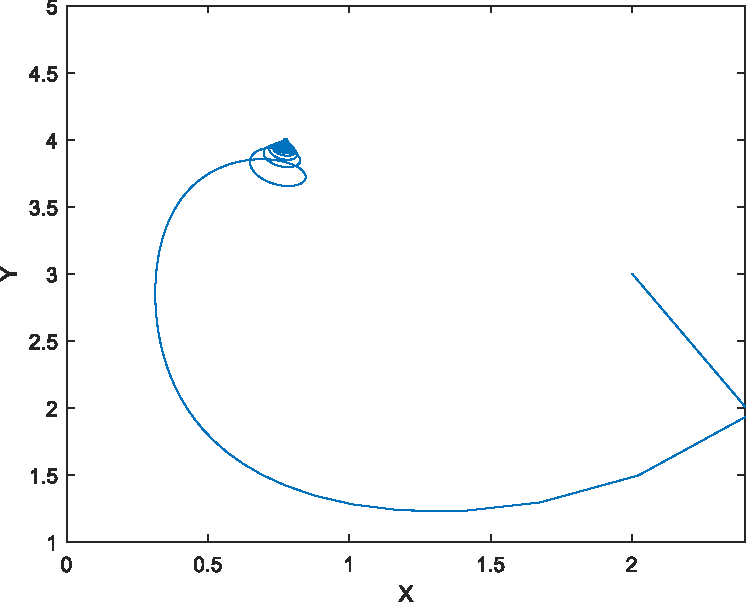
\includegraphics[scale = 0.5]{files/a084.pdf}
    \centering
    \caption{Results when $\alpha=0.84$.}
    \label{fig:2a}
  \end{subfigure}
  \hspace{1cm}
  \begin{subfigure}[H]{0.4\textwidth}
    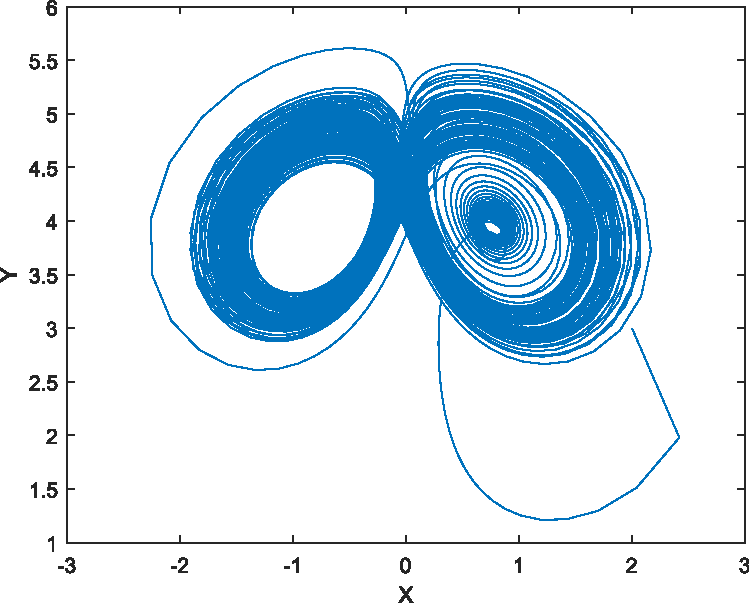
\includegraphics[scale = 0.5]{files/b085.pdf}
    \centering
    \caption{Results when $\alpha=0.85$.}
    \label{fig:2b}
  \end{subfigure}
  \caption{Results for equal fractional order system when $q_1=q_2=q_3=\alpha$.}
  \label{img:equalalpha}
\end{figure}


In figure \ref{img:equalalpha}, the results for equal fractional order are shown. These plots are comparable with the ones showed in Chen's paper \cite{main} in figure \ref{img:equalalpha} (a-b). On the figure \ref{fig:2a}, it can be observed that the plots are slightly different. On the other hand, on figure \ref{fig:2b} the shape is highly similar to the original but, the filling of the graph is not comparable. It would be explained later why this dissimilarities occur. Note that the system changes from a stable trajectory to a chaotic one with a small change on the order. This result will be discussed in the stability analysis section.

\subsubsection{Non-equal fractional order systems}
\begin{figure}[H]
        \centering
        \begin{subfigure}[b]{0.475\textwidth}
            \centering
            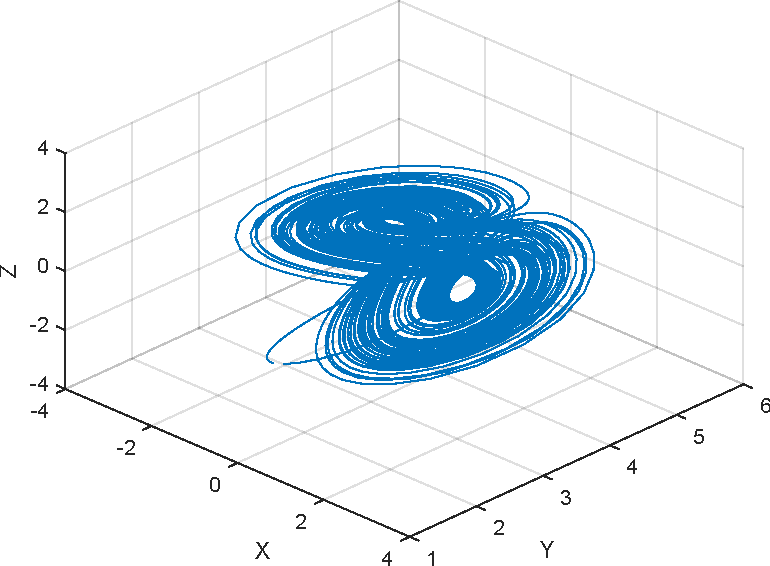
\includegraphics[scale=0.5]{files/a_0_9_1_1.pdf}
            \caption{$q_1=0.90$}    
            \label{fig:3a}
        \end{subfigure}
        \hfill
        \begin{subfigure}[b]{0.475\textwidth}  
            \centering 
            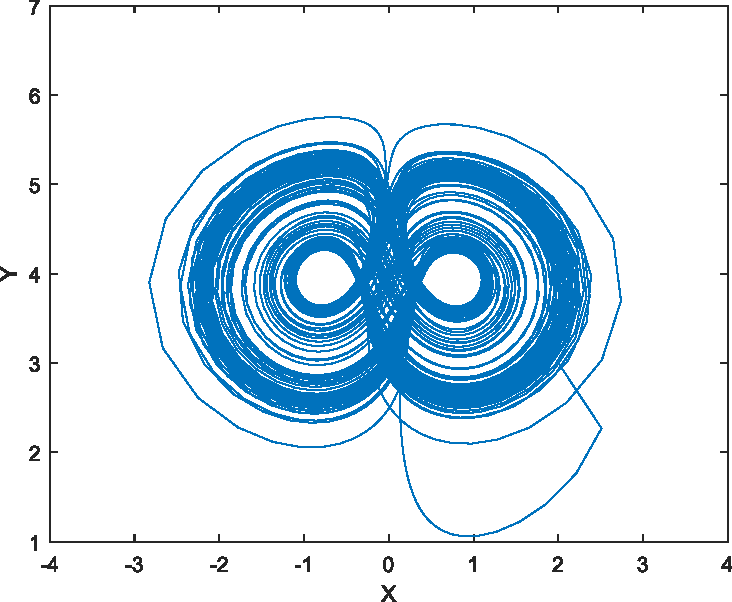
\includegraphics[scale=0.5]{files/b080_1_1.pdf}
            \caption{$q_1=0.80$}  
            \label{fig:mean and std of net24}
        \end{subfigure}
        \vskip\baselineskip
        \begin{subfigure}[b]{0.475\textwidth}   
            \centering 
            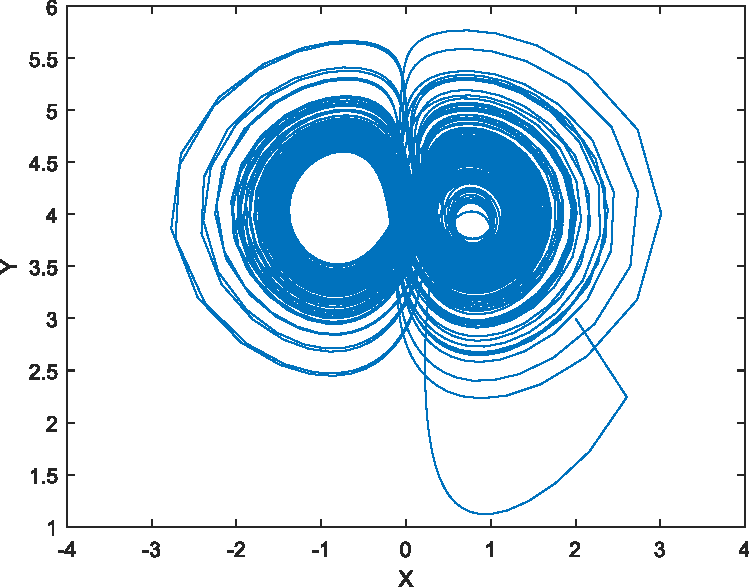
\includegraphics[scale=0.5]{files/c_070_1_1.pdf}
            \caption{$q_1=0.70$}    
            \label{fig:mean and std of net34}
        \end{subfigure}
        \quad
        \begin{subfigure}[b]{0.475\textwidth}   
            \centering 
            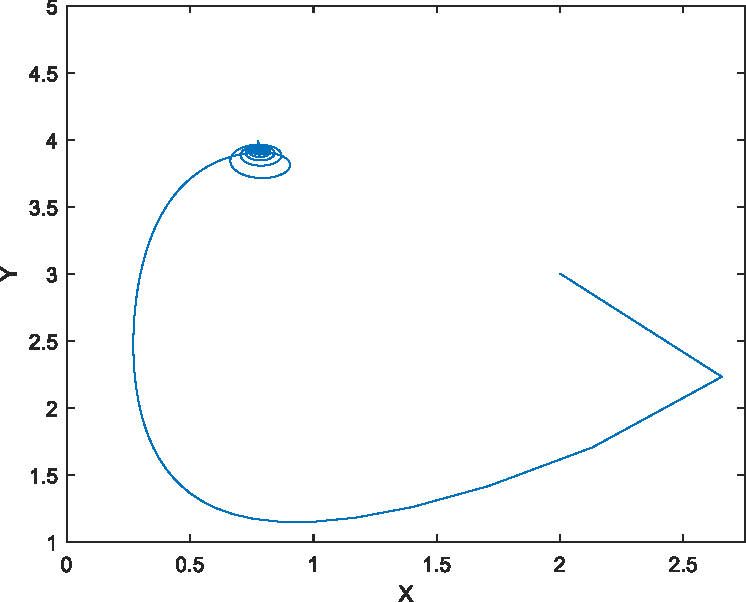
\includegraphics[scale=0.5]{files/d_065_1_1.pdf}
            \caption{$q_1=0.65$}   
            \label{fig:3d}
        \end{subfigure}
        \caption{Results for $q_2=q_3=1$} 
        \label{fig:q2eqq3}
	\end{figure}
In figure, \ref{fig:3a} it was shown the third-dimensional graph instead of a phase-state plane just for illustration purposes. On the remaining it can be seen their similitude with Chen's article.

\begin{figure}[H]
  \centering
  \begin{subfigure}[H]{0.4\textwidth}
    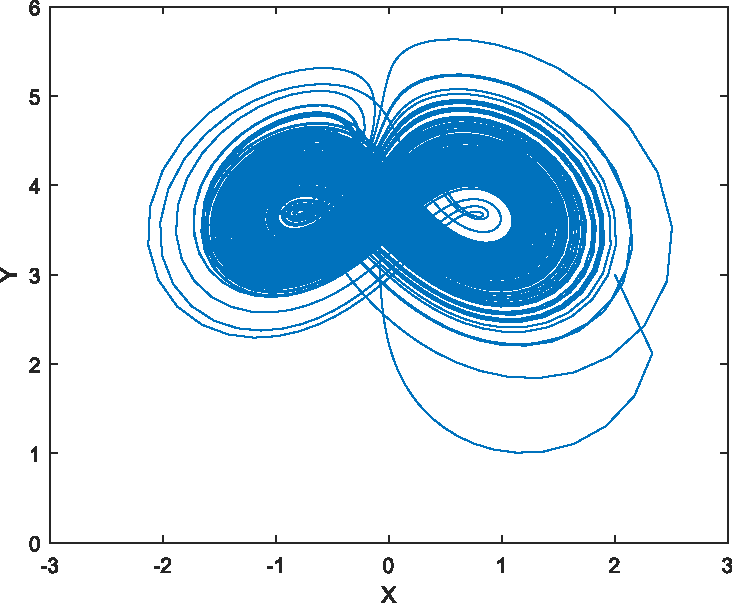
\includegraphics[scale = 0.5]{files/c_1_090_1.pdf}
    \centering
    \caption{$q_2=0.90$.}
  \end{subfigure}
  \hspace{1cm}
  \begin{subfigure}[H]{0.4\textwidth}
    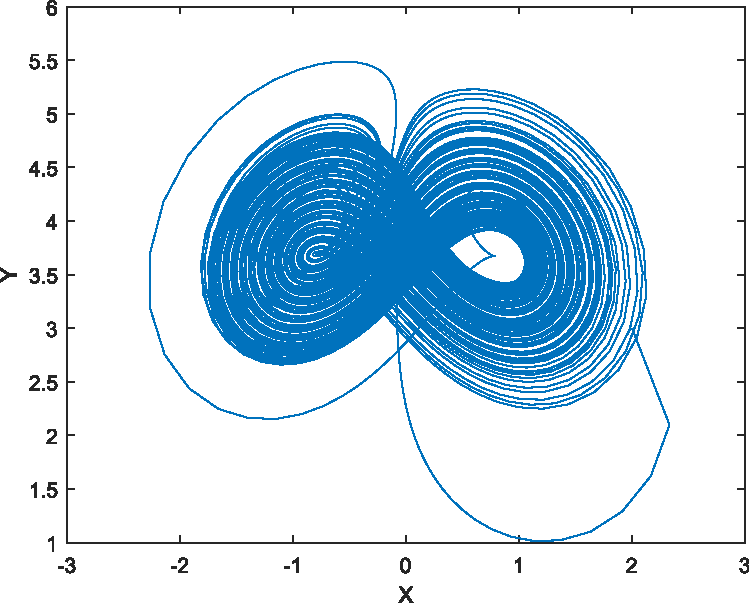
\includegraphics[scale = 0.5]{files/d_1_089_1.pdf}
    \centering
    \caption{$q_2=0.89$.}
    \label{img:messed}
  \end{subfigure}
  \caption{Results for $q_1=q_3=1$.}
  \label{img:q1eqq3}
\end{figure}
Figures \ref{img:q1eqq3}(a-b) are matched to the Figures 3(c-d) in Chen's paper. It can be seen that both graphics are quite different to the ones presented at the original article. Figure \ref{img:messed} graphic has the most considerable difference; even though, it preserves the uniformity of the graph.

\begin{figure}[H]
        \centering
        \begin{subfigure}[b]{0.475\textwidth}
            \centering
            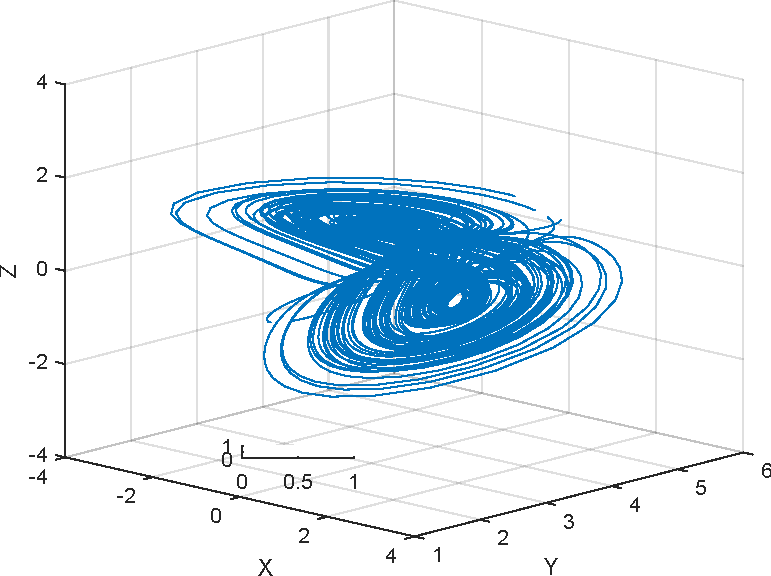
\includegraphics[scale=0.5]{files/a_1_1_090.pdf}
            \caption{$q_3=0.90$}    
            \label{fig:mean and std of net14}
        \end{subfigure}
        \hfill
        \begin{subfigure}[b]{0.475\textwidth}  
            \centering 
            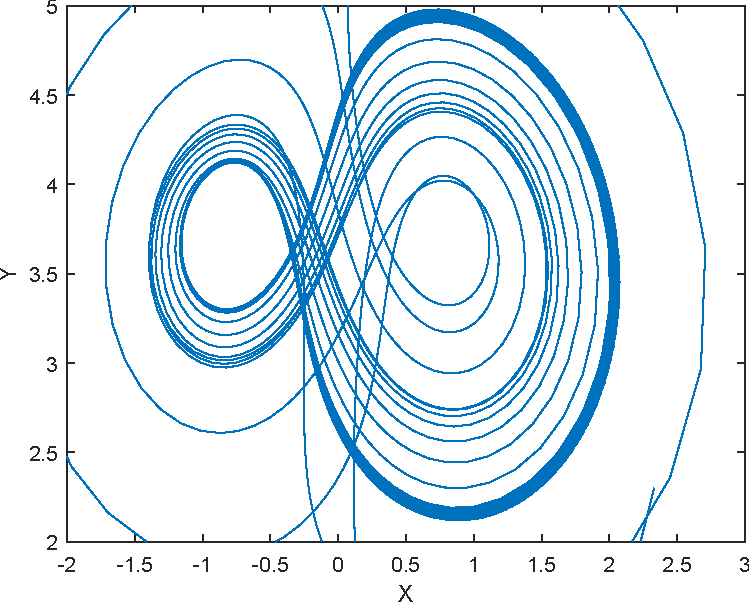
\includegraphics[scale=0.5]{files/b_1_1_080.pdf}
            \caption{$q_3=0.80$}  
            \label{fig:messed2}
        \end{subfigure}
        \vskip\baselineskip
        \begin{subfigure}[b]{0.475\textwidth}   
            \centering 
            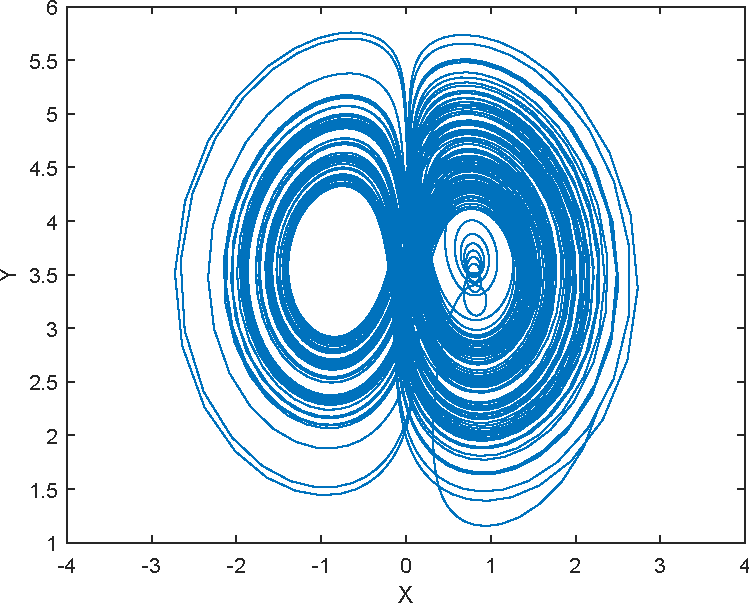
\includegraphics[scale=0.5]{files/c_1_1_05.pdf}
            \caption{$q_3=0.70$}    
            \label{fig:mean and std of net34}
        \end{subfigure}
        \quad
        \begin{subfigure}[b]{0.475\textwidth}   
            \centering 
            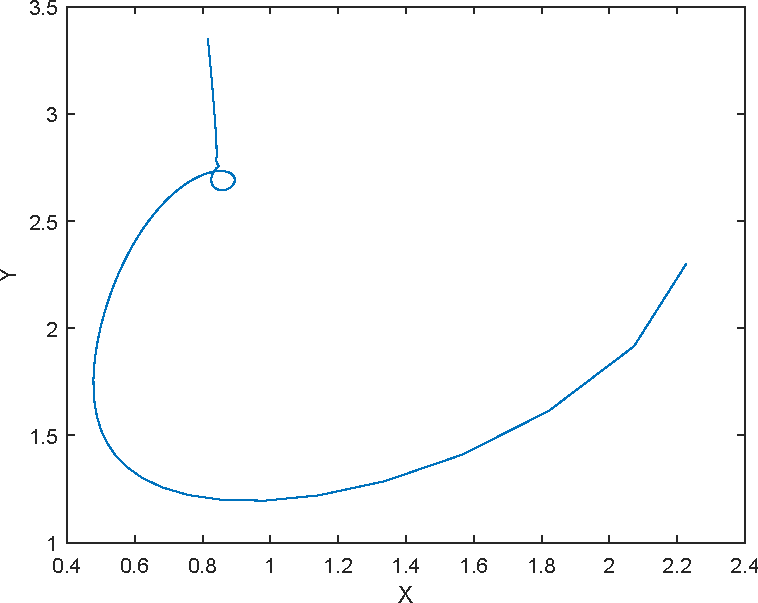
\includegraphics[scale=0.5]{files/d_1_1_020.pdf}
            \caption{$q_3=0.20$}   
            \label{fig:5d}
        \end{subfigure}
        \caption{Results for $q_1=q_2=1$} 
        \label{fig:q1eqq2}
	\end{figure}
    All of the figures depicted at Figure \ref{fig:q1eqq2} are associated to the 5th Figure of Chen. It can be perceived that all of the plots shown above are interchangeable one another with the exception of Figure \ref{fig:messed2}. But, the chart mentioned preserves the shape of the primal.
    
    The differences of the above phase-state portraits could be explained by a number of causes. First of all, Chen does not specifies the time-step nor the upper-bound of the time interval about the simulation that they run; therefore, the lines in the plots can have more iterations thus have more trajectories. On the other hand, Figures \ref{fig:2a}, \ref{fig:3d} or \ref{fig:5d} as they converge to one specific point, it is not as dependent of the time iterations as the rest, therefore their similitude with the original is almost perfect. Another cause for this difference is that the modifications for the Adams-Bashforth-Moulton predictor-corrector, recommended in \cite{diethelm2002predictor}, were not applied for the simulations. It is important to highlight that small changes on the system's order lead to big changes on its behavior.

\subsection{Comparison between Runge-Kutta method and Adams-Bashforth-Moulton predictor-corrector}

In this section, it will be compared the results that both methods give using integer order differentiation. The parameters $a=b=c=0$ were used, therefore the figure \ref{fig:6} can be compared to the second figure of article \cite{integrability}. In the figure \ref{fig:6} the initial conditions were $(x_0,y_0,z_0)=(0,0,2.21)$ and for the next ones, $(x_0,y_0,z_0)=(0,0,1.6)$ was used.

\begin{figure}[H]
  \centering
  \begin{subfigure}[H]{0.4\textwidth}
    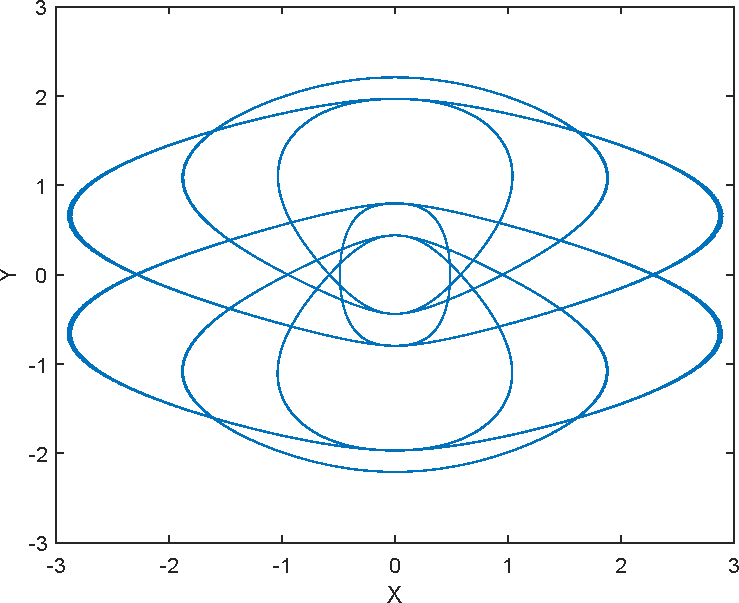
\includegraphics[scale = 0.5]{files/IntegerKutta.pdf}
    \centering
    \caption{Results using Runge-Kutta method.}
  \end{subfigure}
  \hspace{1cm}
  \begin{subfigure}[H]{0.4\textwidth}
    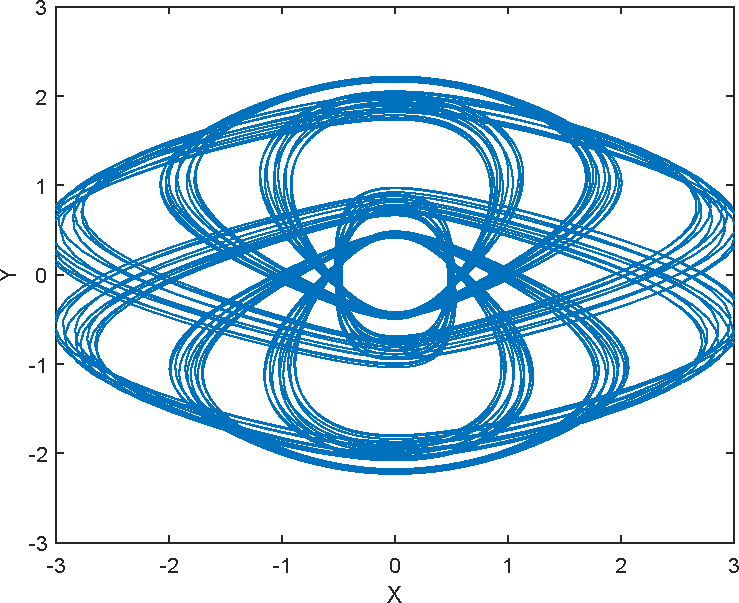
\includegraphics[scale = 0.5]{files/IntegerAdams.pdf}
    \centering
    \caption{Results using Adams-Bashforth-Moulton predictor-corrector.}
    \label{}
  \end{subfigure}
  \caption{Results for integer-order system, i.e. $q_1=q_2=q_3=1$}
  \label{fig:6}
\end{figure}

\begin{figure}[H]
  \centering
  \begin{subfigure}[H]{0.4\textwidth}
    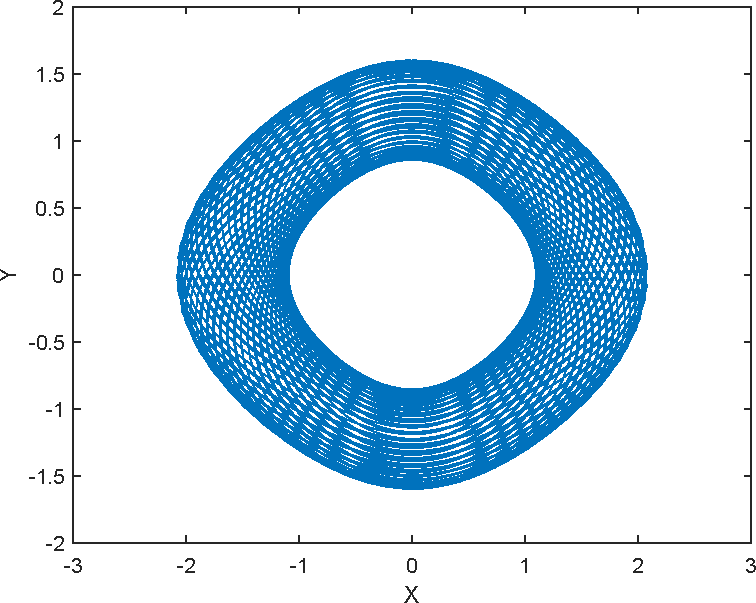
\includegraphics[scale = 0.5]{files/IntegerKutta2.pdf}
    \centering
    \caption{Results using Runge-Kutta method.}
  \end{subfigure}
  \hspace{1cm}
  \begin{subfigure}[H]{0.4\textwidth}
    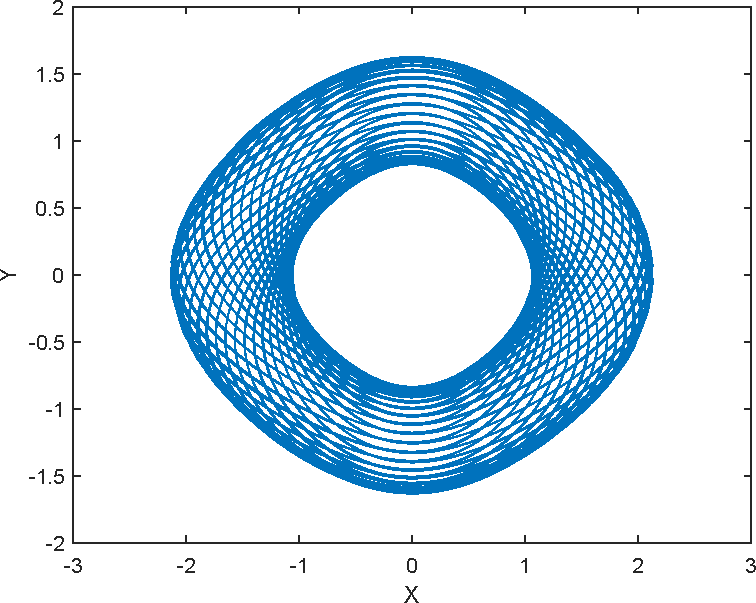
\includegraphics[scale = 0.5]{files/IntegerAdam2.pdf}
    \centering
    \caption{Results using Adams-Bashforth-Moulton predictor-corrector.}
    \label{}
  \end{subfigure}
  \caption{Results for integer-order system, i.e. $q_1=q_2=q_3=1$}
  \label{fig:7}
\end{figure}

It can be shown that both graphs keep the same form independently of the method used; as explained before, the Runge-Kutta is more precise than the other numerical method due to the difference of order. Therefore, every discrepancy of the plots can be explained with the above. 

\section{Stability Analysis}\label{stab}
\subsection{Preliminaries}
For the stability analysis of the fractional order system, the following theorem and definition, proposed and proved in \cite{abd2010chaos}, were applied:
\theoremstyle{definition}
\begin{definition}\label{def:1}
	Given a nonlinear differential system
    \begin{equation}
    	_CD_{0,t}^px(t)=f(x(t)),\quad x(t)\in\mathbb{R}^n
    \end{equation}
    where $x(0)=x_0$, $f(x)$ is continuous, the point $e$ is an equilibrium point of this system, if and only if $f(e)=0$.
\end{definition}
\begin{theorem}\label{theo:1}
Let $x=x^*$ be an equilibrium point of a fractional nonlinear system
\begin{equation}
D^\alpha x = f(x),\quad 0<\alpha<2
\end{equation}
If the eigenvalues of the Jacobian matrix $A = \partial f/\partial x|_{x=x^*}$ satisfy
\begin{equation}
 \min_{i}\left|\arg(\lambda_i)\right|>\alpha \frac{\pi}{2},\quad i=1,2,\dots,n.
\end{equation}
then $x^*$ is asymptotically stable.
\end{theorem}

\subsection{Results}
Analyzing the system shown in \ref{eq:main} and applying the definition \ref{def:1}, the equilibrium points are:
\begin{equation}
	\begin{array}{ll}
		p_1:&X=0\quad Y=\dfrac{1}{b}\quad Z=0\\
    	p_{2,3}:&X=\pm\sqrt{\dfrac{c-b-abc}{c}}\quad Y=\dfrac{1-x^2}{b}\quad Z=-\dfrac{x}{c}\\
	\end{array}
\end{equation}
Now, to analyze the stability of these equilibrium points, the Jacobian of the state variables is needed, thus
\begin{equation}
	J = \left[\begin{array}{ccc}
	Y-a &\quad X 	&\quad 1\\ 
    -2X 	&\quad -b 	&\quad 0\\
    -1 		&\quad 0 	&\quad c
	\end{array}\right]
\end{equation}

For the following simulations, the values for $a$, $b$ and $c$ will be, respectively, $3$, $0.1$ and $1$; $q_1=q_2=q_3=\alpha$ and $0<\alpha<1$ is assumed as well. Therefore, to use theorem \ref{theo:1}, the eigenvalues of the Jacobian matrix are required; using $p_1$ and $p_{2,3}$ as analysis points, the stability will be determined:

With the given values, $p_1=(0,10,0)$ and then respective Jacobian matrix is
\begin{equation}
	J_{p_1} = \left[\begin{array}{ccc}
	7 &\quad 0 	&\quad 1\\ 
    0 	&\quad -0.1		&\quad 0\\
    -1 		&\quad 0 	&\quad -1
	\end{array}\right]
\end{equation}
with eigenvalues $\lambda_1=-0.1$, $\lambda_2\approx 6.8730$ and $\lambda_3\approx-0.8730$. Now, theorem \ref{theo:1} is applied, $\min|\arg(\lambda_1),\arg(\lambda_2),\arg(\lambda_3)|=\min|\pi,\pi,0|=0<\alpha\frac{\pi}{2}$ since $0<\alpha<1$; therefore, according to the theorem, $p_1$ is an unstable equilibrium point.

Following a similar procedure for $p_{2,3}$, it can be obtained that the eigenvalues are $\lambda_1\approx-0.7256$, $\lambda_2\approx0.3128-1.2474i$ and $\lambda_3\approx0.3128+1.2474i$. In this case, we shall analyze the order of the fractional differential equation system ($\alpha$). Given \begin{equation*}
	\min_i|\arg(\lambda_i)|>\alpha\frac{\pi}{2}
\end{equation*}
It can solved for $\alpha$ and obtain a critical value for the order, hence
\begin{equation}
	\alpha < \frac{2}{\pi}\min_i|\arg(\lambda_i)|
\end{equation}
In this case, $\alpha <\frac{2}{\pi}\min_i|\arg(\lambda_1),\arg(\lambda_2),\arg(\lambda_3)| = \frac{2}{\pi}(1.3251)\approx0.8436$. Therefore, if $\alpha<0.8436$ the point $p_{2,3}$ is asymptotically stable; in any other case, is unstable.



\section{Control}
\subsection{Preliminaries}
It is desired to stabilize the system \ref{eq:main} in a periodic orbit (or in a fixed point) $\left(\tilde{x},\tilde{y},\tilde{z}\right)$ using feedback control, as in \cite{abd2010chaos}, hence
\begin{equation}
\begin{array}{ll}
\dfrac{d^{q_1}X}{dt^{q_1}}&=Z+(Y-a)X+u_1(t)\\
\dfrac{d^{q_2}Y}{dt^{q_2}}&=1-bY-X^2+u_2(t)\\
\dfrac{d^{q_3}Z}{dt^{q_3}}&=-X-cZ+u_3(t)\\
\end{array}
\end{equation}

Following the procedure described in \cite{abd2010chaos}, the control functions are defined by
\begin{equation}
	\begin{array}{ll}
		u_1(t)&=-(xy-\tilde{x}\tilde{y})\\
        u_2(t)&=x^2-\tilde{x}^2\\
        u_3(t)&=x-\tilde{x}
	\end{array}
\end{equation}

\subsection{Results}
\subsubsection{Stabilizing the system to a periodic orbit}
For the following simulations, $\alpha=0.9$ will be used. Additionally, the same values from section \ref{stab} for $a$, $b$ and $c$ are used. The solution to the system was obtained with the same Adams-Bashforth-Moulton predictor-corrector, with $N=3000$ and $T=300$. 
	\begin{figure}[H]
        \centering
        \begin{subfigure}[b]{0.475\textwidth}
            \centering
            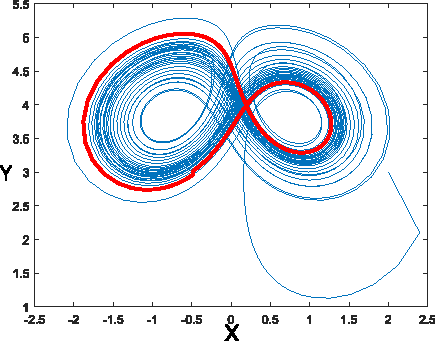
\includegraphics[scale=0.75]{files/OrbitXvsYq0_9.pdf}
            \caption{Uncontrolled phase plane for $XY$ with selected orbit.}    
            \label{fig:unctrlXY}
        \end{subfigure}
        \hfill
        \begin{subfigure}[b]{0.475\textwidth}  
            \centering 
            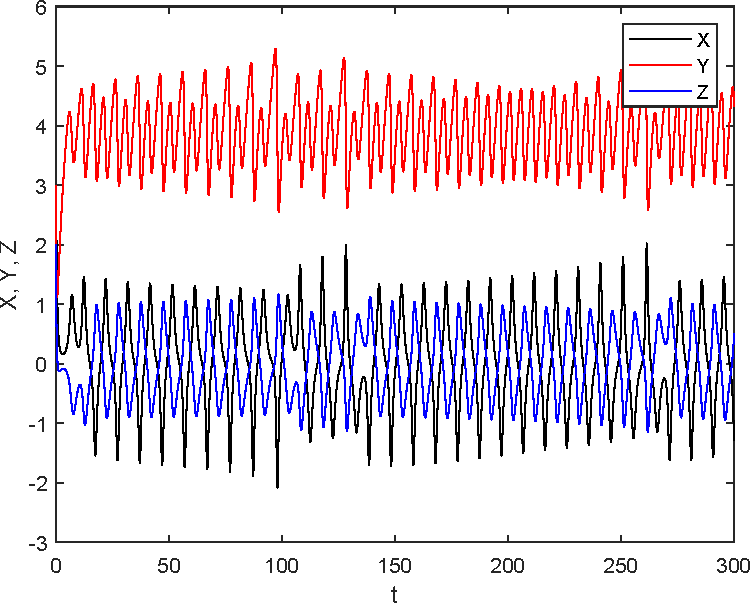
\includegraphics[scale=0.5]{files/OrbitXYZq0_9.pdf}
            \caption{Uncontrolled XYZ against time.}  
            \label{fig:unctrlXYZ}
        \end{subfigure}
        \vskip\baselineskip
        \begin{subfigure}[b]{0.475\textwidth}   
            \centering 
            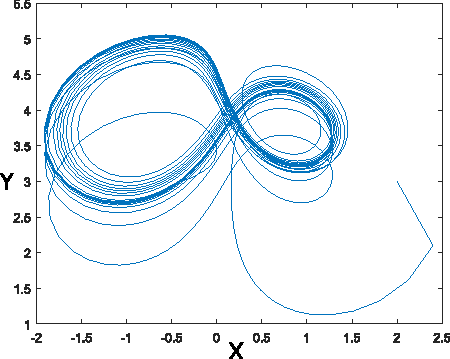
\includegraphics[scale=0.75]{files/ctrlXvsYq0_97.pdf}
            \caption{Controlled phase plane for $XY$.}    
            \label{fig:ctrlXY}
        \end{subfigure}
        \quad
        \begin{subfigure}[b]{0.475\textwidth}   
            \centering 
            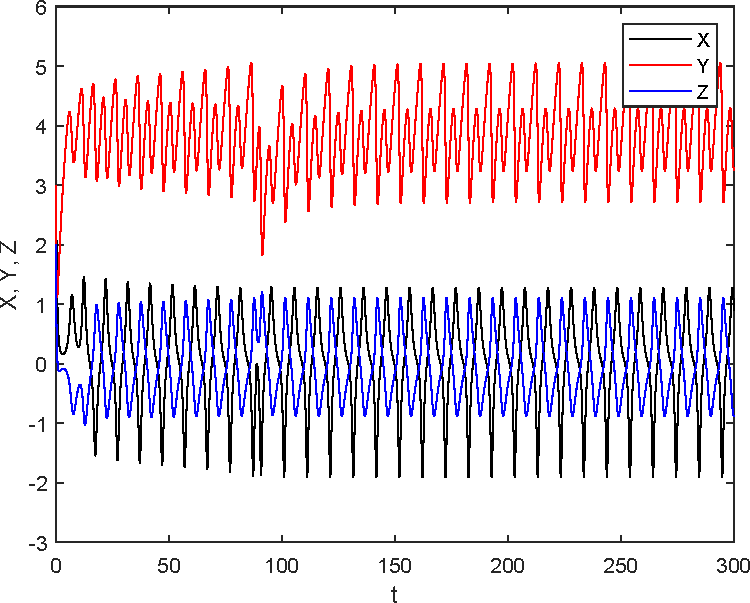
\includegraphics[scale=0.5]{files/ctrlorbitXYZq0_97.pdf}
            \caption{Controlled XYZ against time.}  
            \label{fig:ctrlXYZ}
        \end{subfigure}
        \caption{Results for controlled system in the selected orbit.} 
        \label{fig:o1}
	\end{figure}
      In figure \ref{fig:unctrlXY}, the red path is the selected periodic orbit to stabilize. The period of said orbit is $10.2$, the interval for it is $[78.2,88.4]$. On figure \ref{fig:unctrlXYZ}, the behavior of the state variables through time is shown, note the periodic behavior of these variables through time after the control is applied.
    
    In figure \ref{fig:o1}(a-b), the response for the proposed control is shown. The controller starts when the system fully completes the selected orbit (i.e $t=88.4$), in order to ensure that it remains in a similar shape. Before applying the feedback control, $u_i(t)=0$, $i=1,2,3$. Note that the response is periodic and more consistent compared to the original.

\subsubsection{Stabilizing the system to a fixed point}
In this section, the same $\alpha$, $a$, $b$ and $c$ are used as in the previous simulations, except for the last plot (i.e figure \ref{img:p2}) that $\alpha=0.95$. In order to obtain these results, the controller starts working at $t=22.5$. 
\begin{figure}[H]
  \centering
  \begin{subfigure}[H]{0.4\textwidth}
    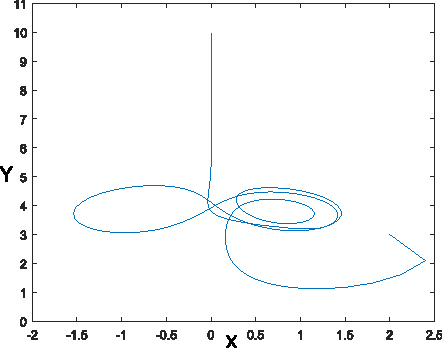
\includegraphics[scale = 0.75]{files/ctrlxvsYFixed0_9.pdf}
    \centering
    \caption{Phase plane for $XY$.}
    \label{fig:p1fixedxy}
  \end{subfigure}
  \hspace{1cm}
  \begin{subfigure}[H]{0.4\textwidth}
    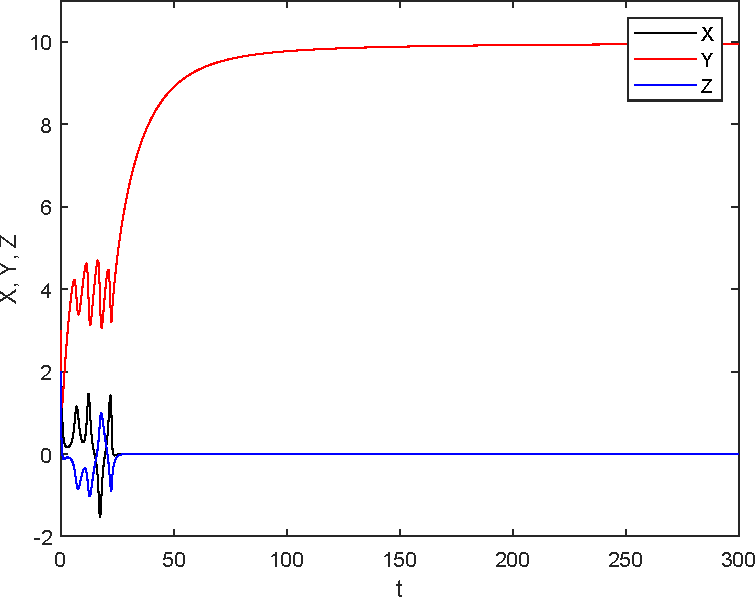
\includegraphics[scale = 0.5]{files/ctrlq0_9.pdf}
    \centering
    \caption{$XYZ$ against time.}
    \label{fig:p1fixedxyz}
  \end{subfigure}
  \caption{Results for controlled system around $p_1$.}
  \label{img:p1}
\end{figure}
In figure \ref{img:p1}, the stabilization for the equilibrium point $p_1=(0,10,0)$ is exhibited. The figure on the left shows how the system converges to this point. The figure on the right shows the behavior of the states variables through time, showing that they also converge to $p_1$.
\begin{figure}[H]
  \centering
  \begin{subfigure}[H]{0.4\textwidth}
    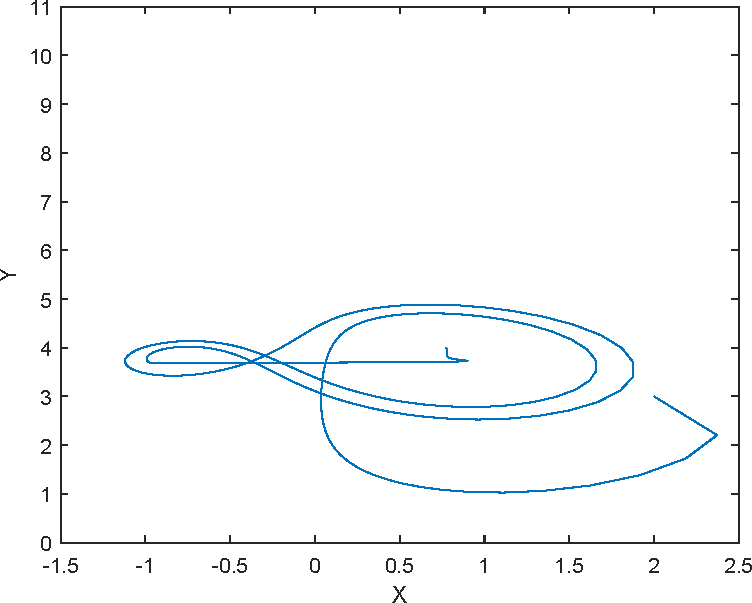
\includegraphics[scale = 0.5]{files/ctrlXvsYFixedq0_95.pdf}
    \centering
    \caption{Phase plane for $XY$.}
    \label{fig:p2fixedxy}
  \end{subfigure}
  \hspace{1cm}
  \begin{subfigure}[H]{0.4\textwidth}
    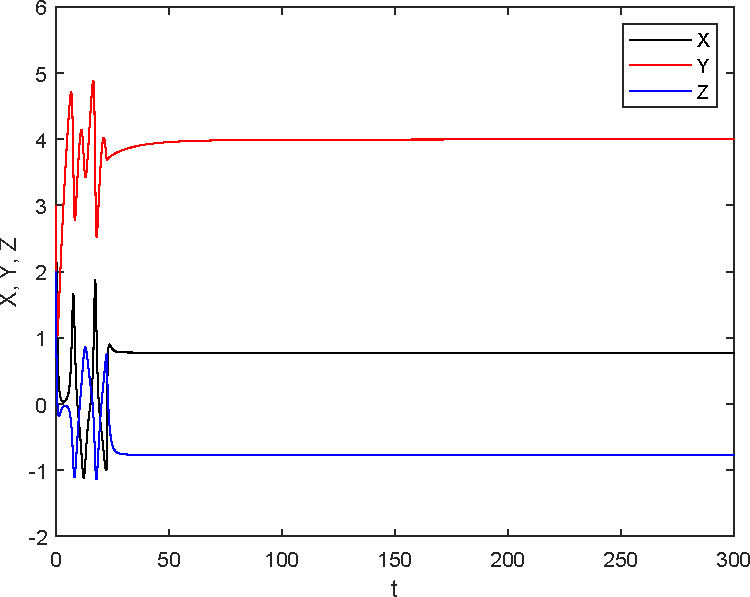
\includegraphics[scale = 0.5]{files/ctrlq0_95.pdf}
    \centering
    \caption{$XYZ$ against time.}
    \label{fig:p2fixedxyz}
  \end{subfigure}
  \caption{Results for controlled system around $p_2$.}
  \label{img:p2}
\end{figure}
In figures \ref{img:p2}(a-b), the equilibrium is achieved around $p_2$, using the same procedure as in the previous simulation. Note that $\alpha=0.95$.

The results obtained in this section can be compared with fixed-point stabilization in Abd-Elouahab \textit{et al.} in \cite{abd2010chaos}.

It can be seen that the system is highly controllable, through the feedback control methodology presented in \cite{abd2010chaos}. There are others types of controllers proposed in the literature for this fractional-order system; see \cite{pan2015multi} or \cite{yang2017modified}.





\section{Sensitivity Analysis}
Recall the fractional dynamic system that is being studied
\begin{equation}\label{eq:mainSystem}
	    \begin{array}{ll}
            \dfrac{d^{\alpha}X}{dt^{\alpha}}&=Z+(Y-a)X\\
            \dfrac{d^{\alpha}Y}{dt^{\alpha}}&=1-bY-X^2\\
            \dfrac{d^{\alpha}Z}{dt^{\alpha}}&=-X-cZ
        \end{array} \qquad \alpha\in(0,1]
\end{equation}
The main goal is measure the sensibility of parameters $a$, $b$ and $c$ as in \cite{guo2016sensitivity}.


For our first simulation, we will be analyzing the commensurate system (i.e same derivative order), $\alpha=0.84$ will be used. The initial values for the parameters are ($\mu_0$): $a_0=3$, $b_0=0.1$ and $c_0=1$. In order to calculate the behavior of $X$, $Y$ and $Z$ respect to $a$, $b$ and $c$, the associated Jacobian matrices are required. Let x be the vector of the state variables and $\mu$ the vector of parameters; hence,
\begin{equation}
	P(t,\mu_0)=\dfrac{\partial f}{\partial x}\Bigr|_{\mu_0} = \left[\begin{array}{ccc}
	Y-3 &\quad X 	&\quad 1\\ 
    -2X 	&\quad -0.1 	&\quad 0\\
    -1 		&\quad 0 	&\quad 1
	\end{array}\right] \qquad\qquad
    Q(t,\mu_0)=\dfrac{\partial f}{\partial \mu}\Bigr|_{\mu_0} = \left[\begin{array}{ccc}
	-X &\quad 0 	&\quad 0\\ 
    0  &\quad -Y 	&\quad 0\\
    0  &\quad 0 	&\quad -Z
	\end{array}\right]
\end{equation}

Let the sensitivity function

\begin{equation}
	S(t) = \dfrac{\partial f}{\partial x}\Bigr|_{\mu_0} = \left[
    \begin{array}{ccc}
		\dfrac{\partial X}{\partial a} &\quad \dfrac{\partial X}{\partial b} &\quad \dfrac{\partial X}{\partial c}\\
        \dfrac{\partial Y}{\partial a} &\quad \dfrac{\partial Y}{\partial b} &\quad \dfrac{\partial Y}{\partial c}\\
        \dfrac{\partial Z}{\partial a} &\quad \dfrac{\partial Z}{\partial b} &\quad \dfrac{\partial Z}{\partial c}
    \end{array}
    \right]\triangleq\left[
    \begin{array}{ccc}
		X_a&\quad  X_b&\quad X_c\\
        Y_a&\quad  Y_b&\quad Y_c\\
        Z_a&\quad  Z_b&\quad Z_c
    \end{array}
    \right]
\end{equation}

Where $S(t)$ contains the new state variables for our system. These variables measure how the state variables change respect to the parameters. Now, the sensitivity equation is defined as

\begin{equation}\label{eq:sensitivity}
	\begin{split}
      \dfrac{d^{0.84}S(t)}{dt^{0.84}} &= P(t,\mu_0)S(t) + Q(t,\mu_0)\\
      &=\left[\begin{array}{ccc}
      Y-3 &\quad X 	&\quad 1\\ 
      -2X 	&\quad -0.1 	&\quad 0\\
      -1 		&\quad 0 	&\quad 1
      \end{array}\right]     \left[\begin{array}{ccc}
          X_a&\quad  X_b&\quad X_c\\
          Y_a&\quad  Y_b&\quad Y_c\\
          Z_a&\quad  Z_b&\quad Z_c
      \end{array}\right]+\left[\begin{array}{ccc}
      -X &\quad 0 	&\quad 0\\ 
      0  &\quad -Y 	&\quad 0\\
      0  &\quad 0 	&\quad -Z
      \end{array}\right]
	\end{split}
\end{equation}

Now, combining the original system and the sensitivity equation, we obtain the new fractional dynamic system
\begin{equation}
	\begin{cases}
	\dfrac{d^{\alpha}X}{dt^{\alpha}}=Z+(Y-3)X, & X(0)=X_0\vspace{1.25mm}\\
    \dfrac{d^{\alpha}Y}{dt^{\alpha}}=1-0.1Y-X^2 & Y(0)=Y_0\vspace{1.25mm}\\
    \dfrac{d^{\alpha}Z}{dt^{\alpha}}=-X-Z & Z(0)=Z_0\vspace{1.25mm}\\
    \dfrac{d^{\alpha}X_a}{dt^{\alpha}}=Z_a-(1+Y_a)X-(3-Y)X_a & X_a(0)=0\vspace{1.25mm}\\
    \dfrac{d^{\alpha}X_b}{dt^{\alpha}}=Z_b+XY_b-(3-Y)X_b & X_b(0)=0\vspace{1.25mm}\\
    \dfrac{d^{\alpha}X_c}{dt^{\alpha}}=Z_c+XY_c-(3-Y)X_c & X_c(0)=0\vspace{1.25mm}\\
    \dfrac{d^{\alpha}Y_a}{dt^{\alpha}}=-0.1Y_a-2XX_a & Y_a(0)=0\vspace{1.25mm}\\
    \dfrac{d^{\alpha}Y_b}{dt^{\alpha}}=-Y-0.1Y_b-2XX_b & Y_b(0)=0\vspace{1.25mm}\\
    \dfrac{d^{\alpha}Y_b}{dt^{\alpha}}=-0.1Y_c-2XX_c & Y_b(0)=0\vspace{1.25mm}\\
    \dfrac{d^{\alpha}Z_a}{dt^{\alpha}}= -X_a -Z_a& Z_a(0)=0\vspace{1.25mm}\\
    \dfrac{d^{\alpha}Z_b}{dt^{\alpha}}= -X_b -Z_b& Z_b(0)=0\vspace{1.25mm}\\
    \dfrac{d^{\alpha}Z_c}{dt^{\alpha}}= -Z-X_c -Z_c& Z_c(0)=0
	\end{cases}
\end{equation}

Adams-Bashforth-Moulton predictor-corrector with $T=1000$, $N=10000$ and $(X_0,Y_0,Z_0)=(2,3,2)$ was used.

\begin{figure}[H]
        \centering
        \begin{subfigure}[b]{0.475\textwidth}
            \centering
            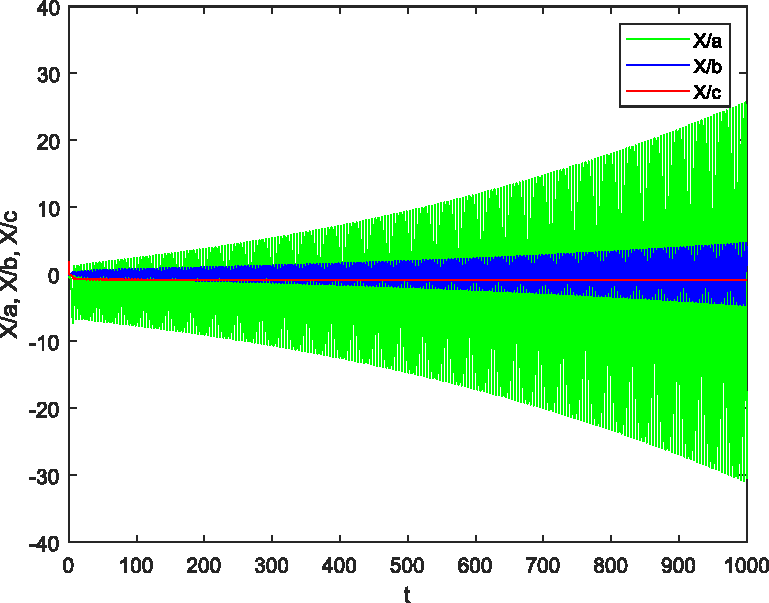
\includegraphics[scale=0.45]{files/dX_084.pdf}
            \caption{Change of X.}    
            \label{fig:dX_084}
        \end{subfigure}
        \hfill
        \begin{subfigure}[b]{0.475\textwidth}  
            \centering 
            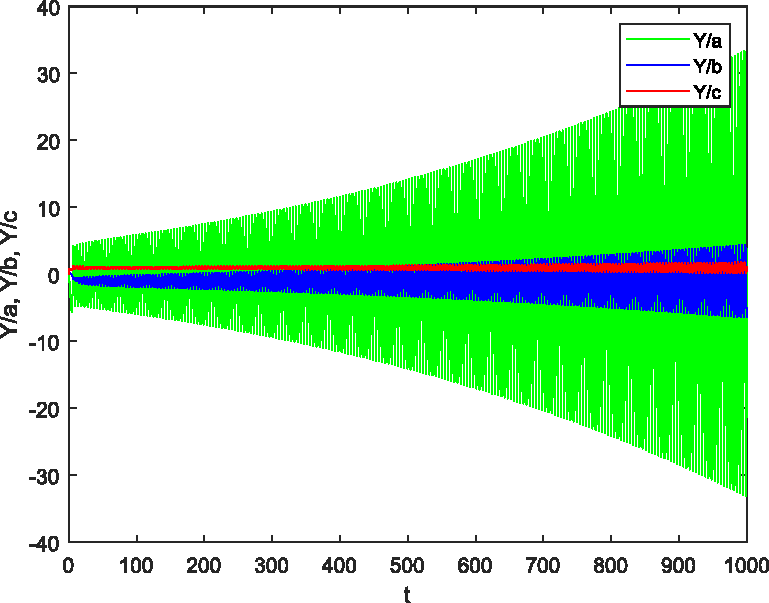
\includegraphics[scale=0.45]{files/dY_084.pdf}
            \caption{Change of Y.}  
            \label{fig:dY_084}
        \end{subfigure}
        \vskip\baselineskip
        \begin{subfigure}[b]{0.475\textwidth}   
            \centering 
            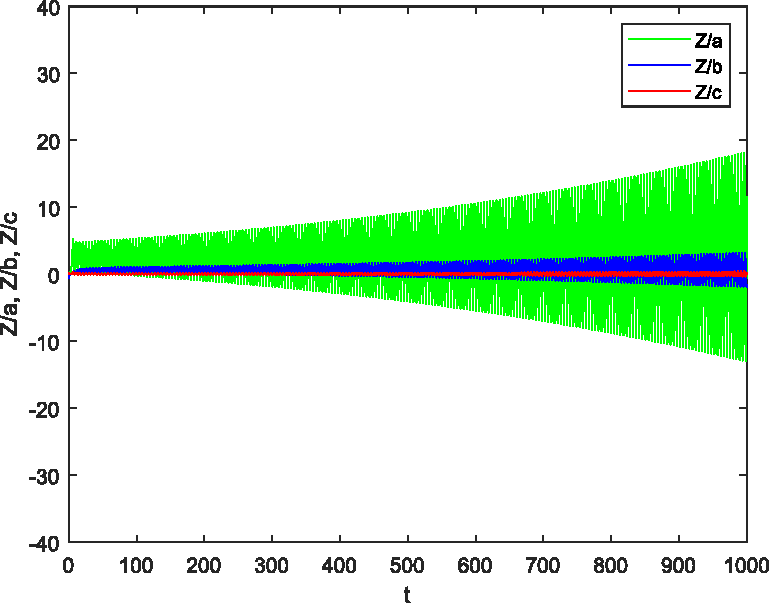
\includegraphics[scale=0.45]{files/dZ_084.pdf}
            \caption{Change of Z.}
            \label{fig:dZ_084}
        \end{subfigure}
        \caption{Changes of state variables respect to parameters.}
        \label{fig:d_084}
	\end{figure}
In figure \ref{fig:d_084}, the results for the sensitivity can be observed for $\alpha=0.84$. Note that, for all state variables, its change respect to $a$ is predominant over $b$ and $c$.

	\begin{figure}[H]
        \centering
        \begin{subfigure}[b]{0.475\textwidth}
            \centering
            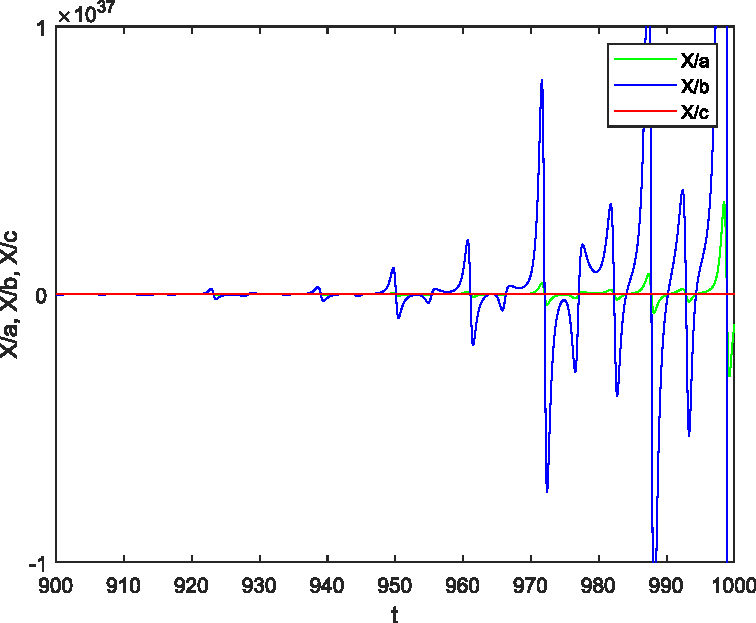
\includegraphics[scale=0.45]{files/dX_085.pdf}
            \caption{Change of X.}    
            \label{fig:dX_085}
        \end{subfigure}
        \hfill
        \begin{subfigure}[b]{0.475\textwidth}  
            \centering 
            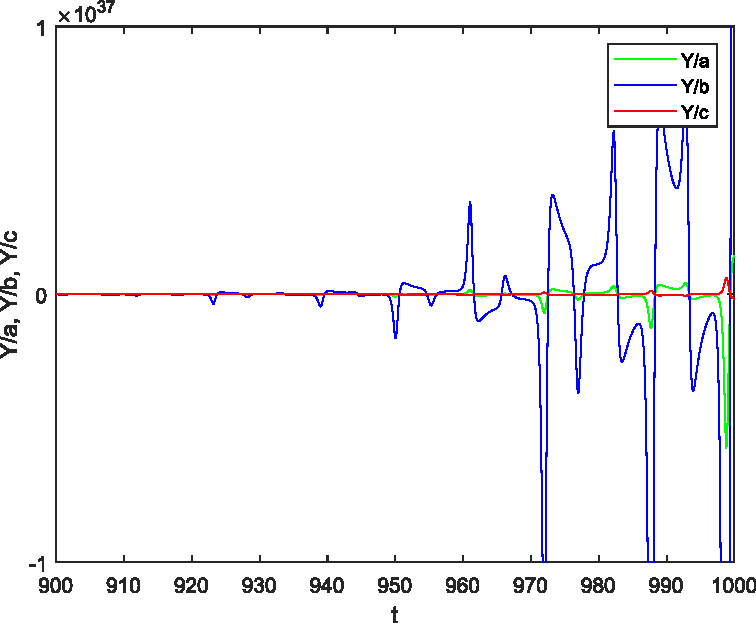
\includegraphics[scale=0.45]{files/dY_085.pdf}
            \caption{Change of Y.}  
            \label{fig:dY_085}
        \end{subfigure}
        \vskip\baselineskip
        \begin{subfigure}[b]{0.475\textwidth}   
            \centering 
            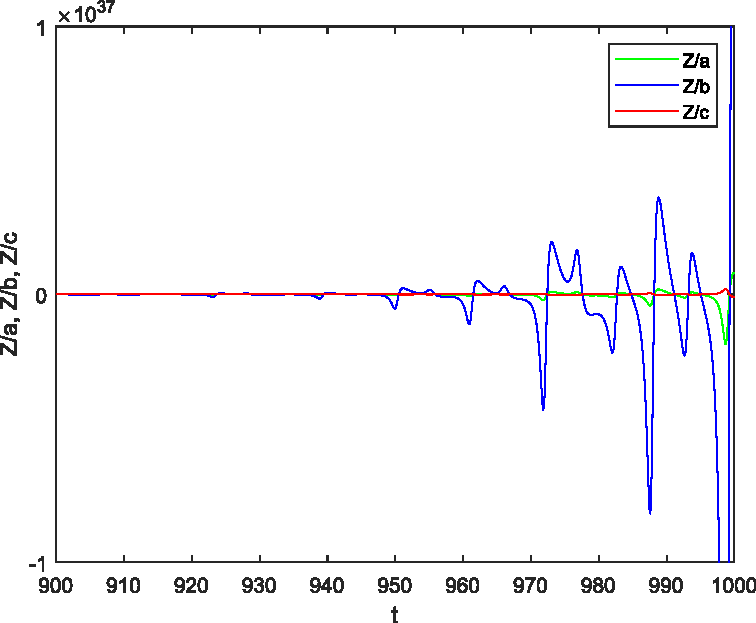
\includegraphics[scale=0.45]{files/dZ_085.pdf}
            \caption{Change of Z.}
            \label{fig:dZ_085}
        \end{subfigure}
        \caption{Changes of state variables respect to parameters.}
        \label{fig:d_085}
	\end{figure}
In figure \ref{fig:d_085}, the results for the sensitivity can be observed for $\alpha=0.85$. Note that, for all state variables, its change respect to $b$ is predominant over $a$ and $c$. Remark: the previous simulation was made with the same $T=1000$ and $N=10000$ as in the one with $\alpha=0.84$, but the plot was made only between $900\leq t\leq1000$ for a better visualization of system's behavior. 

Comparing the results for $\alpha=0.84$ and $\alpha=0.85$, it can be concluded that, in the first simulation, the system is not as sensitive as the one in the second simulation, since the rate of change for $b$ is in the order of $10^{
37}$ and for $a$ in the first one is in the order of $10^1$.

In figure \ref{fig:2a}, it can be seen the phase diagram for $\alpha=0.84$ and in section \ref{stab} it was proved that this system converges to a stable equilibrium point and the sensitivity analysis showed a bounded non-decreasing periodic behavior. 

In figure \ref{fig:2b}, it can be observed the phase diagram for $\alpha=0.85$ and in section \ref{stab} it was proved that this system has unstable equilibrium points and the sensitivity analysis showed a random oscillation, like a noise signal.

This suggests that there could be a relation between the stability of the system and its sensitivity.






\section{Conclusions}
It can be concluded that the graphs coincide in this paper and the Chen's paper using the Adams-Bashforth-Moulton predictor-corrector. Each discrepancy are due to the time-step and the interval of simulation; we suggest that in further work this is more clear so that the results are easier to replicate. In second place, we found that Adams' method can be, to a certain extent, equivalent to the Runge-Kutta method; taking into account, that the orders of both algorithms are different the similitude is a very good approximation. It was also shown that the generalized equations conserve the properties of memory and randomness that are fully necessary to simulate the macro-financial system of China. 

On the other hand, it was seen that the system has three equilibrium points: one of them ($p_1$) will always be unstable, and the other ones ($p_2,p_3$) depend on the system's order ($\alpha$). Additionally, it was found that the system has a critical value for $\alpha = 0.8436$, which is when the stability changes.

A successful control for both equilibrium points and periodic orbits was achieved; showing that the system, regardless of its chaotic behavior, can be stabilized.

Finally, a sensitivity analysis was developed successfully, based on the methods described on literature; based on this results, it could be observed that the sensitivity is highly dependent on the order of the system, yielding different results for each order.

In future work, it could be analyzed the sensitivity for the incommensurate system; furthermore, the system could be analyzed for $\alpha>1$, verifying if the Adams-Bashforth-Moulton predictor-corrector converges for these orders and developing a methodology for both control and sensitivity.









%Bibs
\bibliographystyle{ieeetran}
\bibliography{ref}


\end{document}
